%----------------------------------------------------------------------------------------
%	PACKAGES AND OTHER DOCUMENT CONFIGURATIONS
%----------------------------------------------------------------------------------------

\documentclass[12pt]{article}
\usepackage{polski}
\usepackage[polish]{babel}
\usepackage{babel,blindtext}
\usepackage[utf8]{inputenc}
\usepackage{datetime}
\usepackage{graphicx}
\usepackage{tikz}
\usepackage{amsmath}
\usepackage{multirow}
\usepackage{tabularx}
\usepackage{geometry}
\usepackage{subcaption}
\usepackage{epstopdf}
% Real R
\usepackage{amsfonts}

\bibliographystyle{unsrt}

\geometry{
 	a4paper, 
 	left    = 20mm,
 	right	  = 20mm,
 	top     = 20mm,
 	bottom  = 20mm,
}
 
%----------------------------------------------------------------------------------------
 
%----------------------------------------------------------------------------------------
% DATES
%----------------------------------------------------------------------------------------

\renewcommand{\dateseparator}{.}
\newdate{exercise_date}{08}{03}{2016}


% dodatkowe typy kolumn tabel

% flush left fixed width:
\newcolumntype{L}[1]{>{\raggedright\arraybackslash}p{#1}}

% center fixed width:
\newcolumntype{C}[1]{>{\centering\arraybackslash}p{#1}}

% flush right fixed width:
\newcolumntype{R}[1]{>{\raggedleft\arraybackslash}p{#1}}

%----------------------------------------------------------------------------------------

%----------------------------------------------------------------------------------------
% TIKZ PACKAGES
%----------------------------------------------------------------------------------------

\usetikzlibrary{arrows}

%----------------------------------------------------------------------------------------

\begin{document}
 
\begin{titlepage}

\newcommand{\HRule}{\rule{\linewidth}{0.5mm}}
% Defines a new command for the horizontal lines, change thickness here

\center
% Center everything on the page
 
%----------------------------------------------------------------------------------------
%	LOGO SECTION
%----------------------------------------------------------------------------------------


\includegraphics[width=6cm]{../res/img/logo.png}\\[1cm]
% Include a department/university logo - this will require the graphicx package
 
%----------------------------------------------------------------------------------------
 
%----------------------------------------------------------------------------------------
%	HEADING SECTIONS
%----------------------------------------------------------------------------------------

\textsc{\LARGE Akademia Górniczo-Hutnicza \\[0.2cm]
im. Stanisława Staszica w Krakowie}\\[1.5cm]
% Name of your university/college

\textsc{\Large Optymalizacja w systemach sterowania}\\[0.5cm]
% Major heading such as course name

%----------------------------------------------------------------------------------------
%	TITLE SECTION
%----------------------------------------------------------------------------------------

\HRule \\[0.5cm]
{ \huge \bfseries Implementacja asystenta pasa ruchu na Xilinx Zynq}\\[0.3cm]
% Title of your document
\HRule \\[1.5cm]

\flushright
\Large \emph{Prowadzący:}\\
dr inż. Tomasz \textsc{Kryjak}\\[1cm]
\Large \emph{Autorzy:}\\
Konrad \textsc{Adasiewicz}\\[0.1cm]        % Your name
Anna \textsc{Musiał}\\[0.1cm]  % Your name
Filip \textsc{Kubicz}\\[3cm]
% Authors


%----------------------------------------------------------------------------------------
%	DATE SECTION
%----------------------------------------------------------------------------------------
% Data wykonania ćwiczenia: \\
% {\large \displaydate{exercise_date}}\\[1cm]


\vfill % Fill the rest of the page with whitespace

\end{titlepage}
\section{Wstęp}

Jazda samochodem jest niebezpieczna. W Polsce w 2015 roku miało miejsce 32 967 wypadków drogowych, w których zginęło 2 938 osób \cite{policja}. 82,8\% wypadków było spowodowanych przez kierowców.
Jednym z systemów, który może poprawić bezpieczeństwo na drogach jest ostrzeżenie o zmianie pasa ruchu. Ostrzegawczy sygnał dźwiękowy lub nawet aktywna zmiana toru jazdy samochodu może powstrzymać zasypiającego lub nieuważnego kierowcę przed zjechaniem do rowu, potrąceniem pieszego na poboczu czy spowodowaniem kolizji z innymi samochodami.

W celu rozpoznania pasów ruchu i położenia samochodu względem jezdni wykorzystaliśmy wykrywanie krawędzi metodą Canny, a następnie transformatę Hougha na otrzymanym obrazie binarnym w celu znalezienia linii malowań zbliżonych do prostych. W dalszej części opisano model programowy w OpenCV, model stałoprzecinkowy C++ oraz opis sprzętu na platformę Xilinx Zynq w języku Verilog.


\section{Wykrywanie pasów ruchu - przegląd artykułów naukowych}

Projekt miał charakter badawczo-implementacyjny. Do uzyskania obrazu binarnego krawędzi wykorzystaliśmy algorytm Canny opracowany w pracy inżynierskiej \cite{inz-canny}. Następnie należało zdecydować w jaki sposób rozpoznawać pasy ruchu i jak wybrany algorytm zrealizować w torze wizyjnym na platformie Xilinx Zynq-7000.

\begin{wrapfigure}{r}{0.5\textwidth}
\vspace{-20pt}
  \begin{center}
    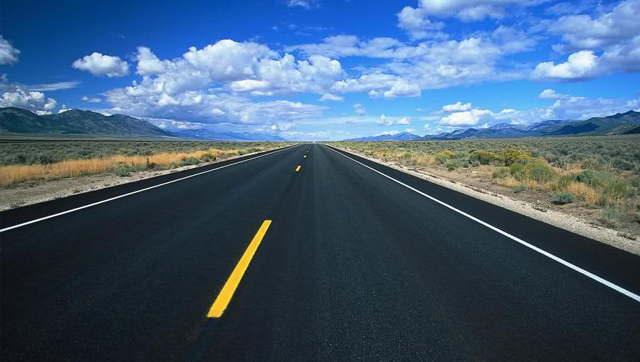
\includegraphics[width=0.4\textwidth]{img/road.jpg}%{./Pictures/mainscreen1.png}
    \caption{Widok z przedniej kamery w samochodzie}
    \label{rys:road}
  \end{center}
  \vspace{-20pt}
  \vspace{1pt}
\end{wrapfigure} 

Do wykrywania pasów ruchu wybraliśmy transformatę Hougha, jako że pasy drogowe widziane z przedniej kamery w aucie najczęściej są zbliżone do linii prostych. Przykład analizowanego obrazu przedstawia rysunek \ref{rys:road}.

Transformata Hougha jest złożoną operacją, którą trudno zrealizować w czasie rzeczywistym na systemie procesorowym. Wpływa na to konieczność wykonania obliczeń dla każdego kąta $\theta$ dla każdego piksela obrazu (lub przynajmniej pikseli należących do krawędzi). Przy obliczaniu transformaty Hougha dla kątów co 1\degree  dla obrazu HD 1280x720 pikseli, trzeba wykonać 331 776 000 mnożeń dla każdej ramki.
Praca \cite{hardware-accelerator} podaje sposób zrównoleglenia obliczeń arytmetycznych w transformacie Hougha na układzie FPGA.


\begin{figure}[!htb]
  \begin{center}
    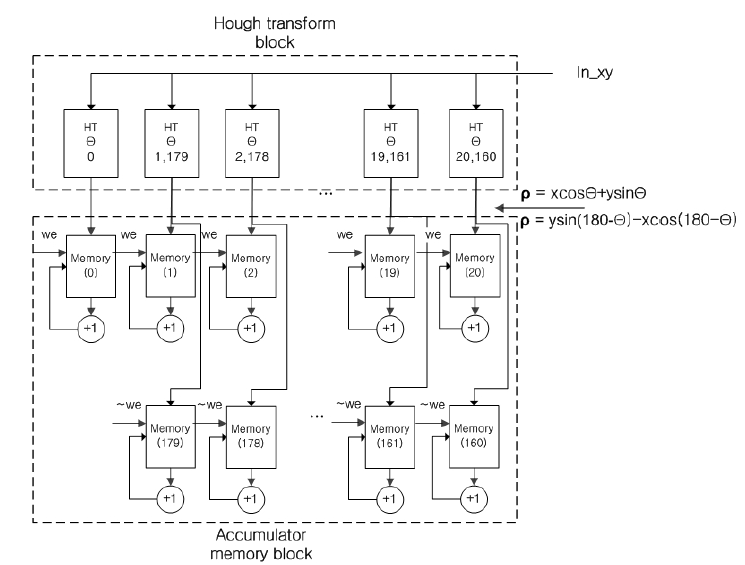
\includegraphics[width=0.9\textwidth]
    {img/hough-accelerator.PNG}
  \end{center}
  \caption{Architektura obliczeniowa transformaty Hougha w pracy \cite{hardware-accelerator}}
  \label{rys:accelerator}
\end{figure}

\newpage

W pracy \cite{kapruziak} opisano 

\blindtext

%\begin{figure}[!htb]
%  \begin{center}
%    \includegraphics[width=14.5cm,trim=1.6cm 6.9cm 1.7cm 8.5cm,clip]
%    {img/exp_omega.pdf}
%  \end{center}
%  \caption{Eksperyment wyznaczenia charakterystyk prędkości śmigieł od napięcia na silnikach przy zablokowanych osiach}
%  \label{plot:exp1}
%\end{figure}






\section{Opis algorytmu}



\subsection{Wykrywanie krawędzi metodą Canny}

Zacytować pracę magisterską, nie opisujemy chyba?

\subsection{Rozpoznawanie linii - transformata Hougha}

Hough

%\begin{figure}[!htb]
%  \begin{center}
%    \includegraphics[scale=0.85]{img/maglev.PNG}
%    \caption{Stanowisko laboratoryjne magnetycznej lewitacji}
%  \end{center}
%  
%  \label{rys:maglev}
%\end{figure}

%\begin{equation} \label{maglev_rown}
%  \begin{cases}
%    \dot{x}_1 & = x_2 \\
%    \dot{x}_2 & = -e^{-x_1} \cdot x_3^2 + 1 \\
%    \dot{x}_3 & = -cx_3 + u
%    \end{cases}
%\end{equation}
%

%Współczynniki przeskalowania zebrano w tabeli.
%
%\begin{table}[!htb]
%  \centering
%  \begin{tabular}{|c|l|l|}
%  \hline
%  Współczynnik & Wartość \\
%  \hline
%  $\alpha$ & $0,00773746 m$ \\
%  \hline
%  $\beta$ & $0,275507681 m/s$ \\
%  \hline
%  $\gamma$ & $0,28890446065998 A$ \\
%  \hline
%  $\xi$ & $0,2808437120924$ \\
%  \hline
%  $\eta$ & $10,28701901522286 A/s$ \\
%  \hline
%  \end{tabular}
%  \caption{Parametry przeskalowania modelu}
%  \label{tab:idf}
%\end{table}



\section{Model programowy transformaty Hougha}

\blindtext

\subsection{Model funkcjonalny z użyciem OpenCV}

\texttt{hough()}

Do budowy modelu funkcjonalnego użyte zostały funkcje biblioteki OpenCV:\\*
\texttt{void Canny(InputArray image, OutputArray edges, double threshold1, double threshold2, int apertureSize=3)} \\*

gdzie \\*
\texttt{image} – obraz wejściowy \\*
\texttt{edges} – wyjściowy obraz do detekcji krawędzi, \\*
\texttt{threshold1} – pierwszy próg binaryzacji,\\*
\texttt{threshold2} – drugi próg binaryzacji,\\*
\texttt{apertureSize} – rozmiar maski użytej w funkcji \texttt{Sobel()}.\\*

\texttt{void HoughLines(InputArray image, OutputArray lines, double rho, double theta, int threshold, double srn=0, double stn=0 )}
\texttt{image} – binarny obraz wejściowy,
\texttt{lines} – wyjściowy wektor linii; każda reprezentowana jest przez dwa elementy – $\rho$ i $\theta$
\texttt{rho} – krok dla odległości $\rho$ w pikselach
\texttt{theta} – krok dla kąta $\theta$ w radianach
\texttt{threshold} – próg głosów, które musi osiągnąć linia aby została zwrócona.


screeny z programu

% 3 obrazki obok siebie
\begin{figure}[!htb]
\minipage{0.32\textwidth}
  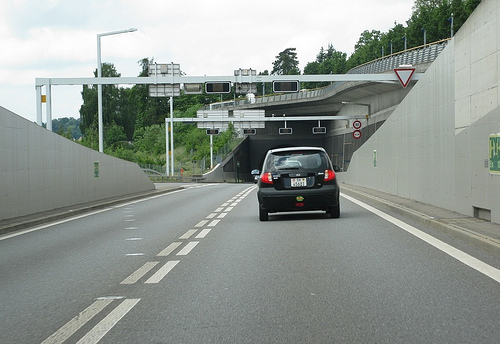
\includegraphics[width=\linewidth]{img/road4.jpg}
  \caption{Obraz z kamery}\label{fig:awesome_image1}
\endminipage\hfill
\minipage{0.32\textwidth}
  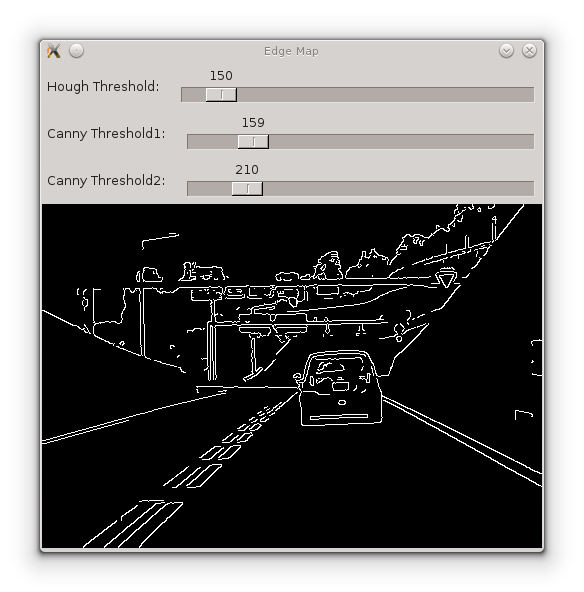
\includegraphics[width=\linewidth]{img/canny_screen.png}
  \caption{Krawędzie znalezione metodą Canny}\label{fig:awesome_image2}
\endminipage\hfill
\minipage{0.32\textwidth}%
  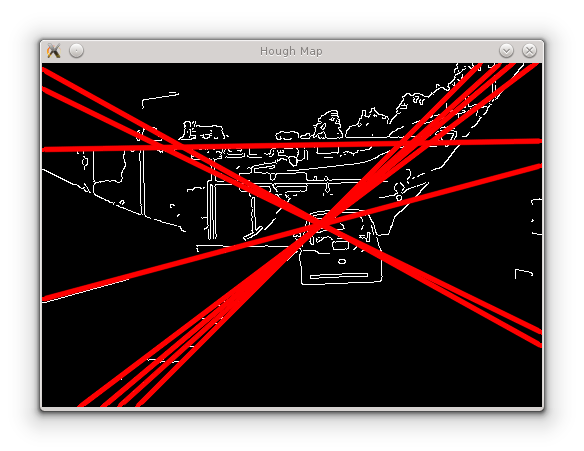
\includegraphics[width=\linewidth]{img/hough_screen.png}
  \caption{Linie wybrane przez transformatę Hougha z głosowaniem}\label{fig:awesome_image3}
\endminipage
\end{figure}

\blindtext

%
%\begin{figure}[!htb]
%\centering
%\includegraphics[scale=1]{img/start2.png}
%\caption{Rozwiązanie przed optymalizacją z wektorem przełączeń $\tau = [0.015, 0.035, 0.055]$}
%\label{rys:start1}
%\end{figure}

\newpage
\subsection{Model stałoprzecinkowy w języku C++}

Klasa \texttt{fp.h}

\begin{figure}[!htb]
\centering
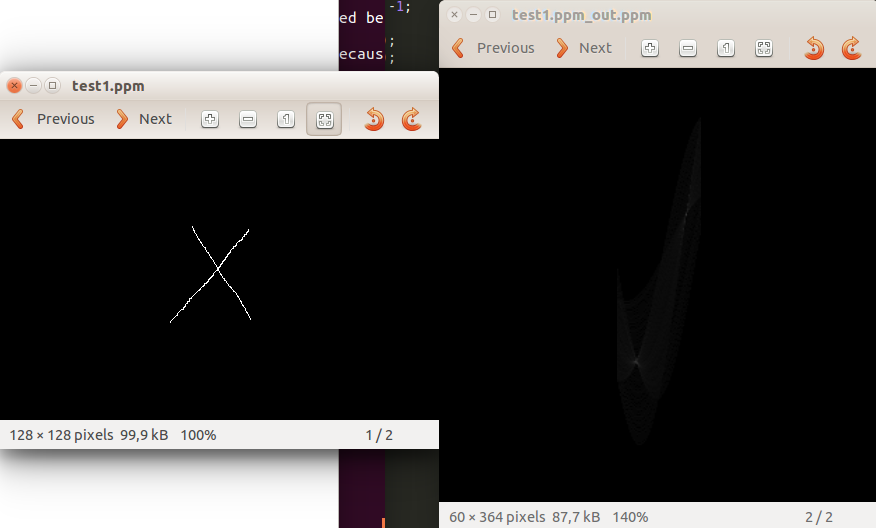
\includegraphics[scale=0.75]{img/fixed.png}
\caption{Wynik działania funkcji \texttt{Hough()} dla liczb stałoprzecinkowych}
\label{rys:fp}
\end{figure}


\section{Realizacja modułu Hough w sprzęcie}


%
%
%\begin{figure}[!htb]
%\centering
%\includegraphics[scale=1]{img/start2.png}
%\caption{Rozwiązanie przed optymalizacją z wektorem przełączeń $\tau = [0.015, 0.035, 0.055]$}
%\label{rys:start1}
%\end{figure}
%



\section{Wnioski}

Zybo ...

Zabrakło czasu, aby poszczególne moduły implementacji sprzętowej połączyć ze sobą i wykorzystać do wykrywania linii.

\subsection{Możliwe ulepszenia}


\bibliography{chapters/Bibliografia}

\end{document}